\section{Samostatná práce člena týmu\ --\ Vít Hrbáček}
\label{sec:individual_work_vit}

\subsection{Výběr tématu, popis provedeného průzkumu s uživatelem, analýza uživatelských potřeb a klíčových problémů, navržená sada změn}

\subsubsection*{Výběr tématu}

{\large Můj hlavní návrh:}

Plugin pro vložení fóra do předešlého školského informačního systému VUT FIT


{\noindent \large Vedlejší návrh:}

Informační systém pro správu promítání kina a zakoupení vstupenek uživatelem

\subsubsection*{Provedený průzkum}

{ \noindent \large Rezervační systém pana doktora Bidla pro domluvení konzultací:}

Domluvil jsem si osobní konzultace s doktorem Bidlem ohledně probrání jeho uživatelského pohledu rezervačního systému, takže jsem měl to štěstí zrovna vyzkoušet jeho systém v praxi. Doktor Bidlo mi na konzultacích vyprávěl, že v minulosti domlouval konzultace přes emaily. Fungovalo to tak, že vypsal všechny termíny, kdy je k dispozici a student také. Bylo občas složité se přes maily domluvit. Vytvořil si proto na míru aplikaci, která mu s tím pomohla. 
\noindent\emph{ \ref{fig:Vit_n}.}

\begin{figure}[htbp]
    \centering
    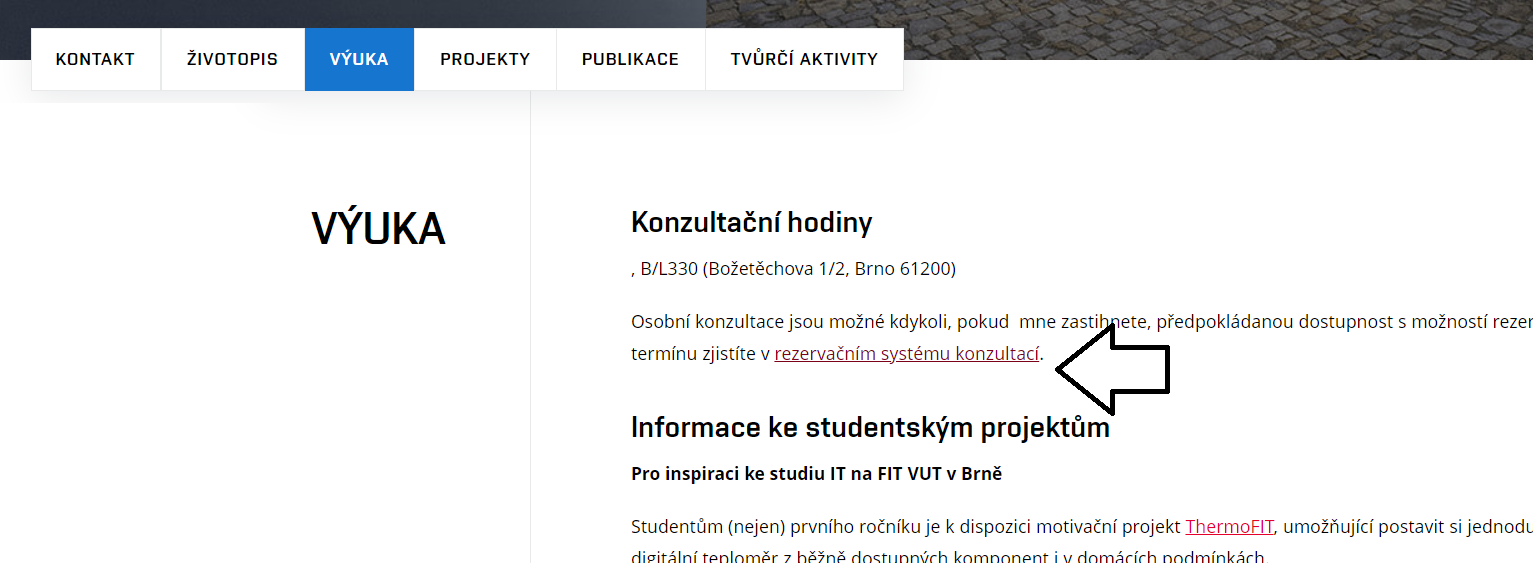
\includegraphics[width = \textwidth]{doc/latex/fig/vit/1.png}
    \caption{Defaultní stránka pro hledání informací o konzultacích zaměstnance fakulty}
    \label{fig:Vit_n}
\end{figure}


\subsubsection*{Analýza potřeb a klíčových problémů}

Program slouží všem uživatelům k tomu, aby studentům zprostředkovával informace o dostupnosti termínů na doktorovy konzultace. Na veřejných stránkách vedle výpisu termínu konzultací má odkaz na stránku s rezervacemi konzultací.

\subsubsection*{Navržené změny}
Pan doktor byl velice šikovný. Jako bývalý student znal potřeby svých studentů a sám sebe, tak si systém vytvořil, jak by měl vypadat podle svých vlastních představ. Díky tomu není moc vylepšení uživatelského rozhraní. Jediné, na co jsme přišli bylo, že pro uživatele je neintuitivní napsat svůj login (identifikátor studenta na fakultě doktora Bidla) do políčka představující volný termín. Jako vhodné vylepšení lze navrhnout změnit políčko na tlačítko po kterém se zobrazí vyskakovací okno, kde by uživatel vypsal svůj login. Doktor Bidlo vybral login jako jedinou potřebnou informaci, kterou musí student zapsat kvůli tomu, že student nemusí zadat mnoho a doktor Bidlo jednoduše z něho zjistí studentovo jméno a e-mailovou adresu.

\newpage
\subsection{Popis současného řešení\ --\ jaké nástroje uživatel používá, \\
popř. obrázky/screenshoty současného řešení/reálné situace}

\noindent\emph{Výměna rozvrhů} 
\begin{itemize}
    \item[+] Dostačující v případě mírného zájmu o konzultace
    \item[--] Časově náročné
    \item[--] Administračně náročnější
	\item[>] Někteří vyučující mají pevně vypsané konzultační hodiny. Řeší to snazší organizaci, ale v praxi nikdo nemusí přijít.
\end{itemize}

Rezervační systém doktora Bidla je mnohem efektivnější. Stránka obsahuje rozvrhy pana Bidla v několika následujících týdnech. Volné termíny, kdy je možné ho fyzicky potkat na škole jsou zeleně a termíny, kdy je dostupný online, jsou žluté. Student si může vybrat jakýkoliv dostupný termín. 

\begin{figure}[htbp]
    \centering
    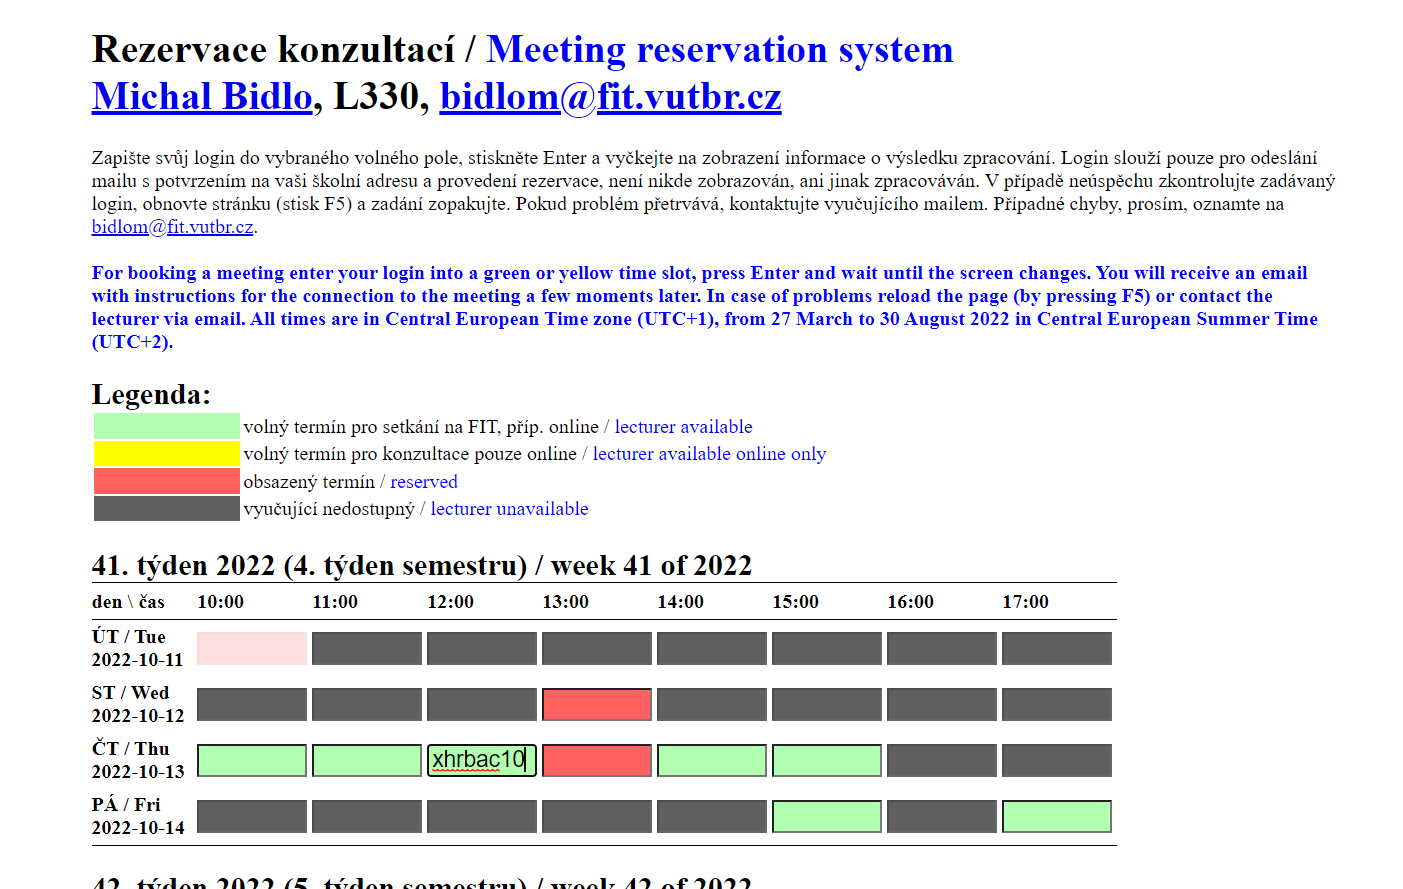
\includegraphics[width = \textwidth]{doc/latex/fig/vit/2.png}
    \caption{Snímek obrazovky Bidlova rezervačního systému}
    \label{fig:Vit_k}
\end{figure}

Termín se rezervuje zapsáním školního loginu do volného pole\\ a~zmáčknutím enter.
Výhodou je nutnost odeslat minimum dat a netřeba se registrovat a přihlašovat na stránku. Nevýhodou je již zmíněné neintuitivní pochopení systému. Je potřeba si přečíst nápovědu výše pro pochopí, co se od uživatele očekává. Zapsaní studenti jsou schválně na stránce anonymní. Po odentrování se zobrazí hláška o úspěchu či neúspěchu rezervace. Líbí se mi, že je zde i odkaz na mapu s umístěním místnosti, kde se konzultace konají. Je to totiž přesně informace, kterou by student o doktorovi jinak musel vyhledávat. Zároveň systém pošle dva emaily. První je potvrzení na studentův email, který zjistil podle jeho školního loginu, a upozornění o nové konzultaci na email pana doktora. Panu doktorovi vyhovuje, že nemusí procházet denně další stránku, ale pípne mu na telefonu, že mu někdo přijde na konzultace. Hodí se to i na konzultacích na poslední chvíli. Uživatel může zadat konzultaci na brzký termín a doktor se o ní snadno doví. 
Termín si může student zrušit pomocí odkazu v emailu. Aplikace, mimo emailu zaslanému panu doktorovi, nemá žádné jiné uživatelské rozhraní. Pan doktor může v případě potřeby přímo studentský login vepsat. Pan doktor používá systém tak, že mu přijde notifikace na nový email. Studenti zmíněným způsobem. Z pohledu studenta, který si konzultace rezervoval mi program vyhovoval. V době koronavirusu zaslal software s mírnými úpravami i jiným přednášejícím, ale nikdo neprojevil zájem.

\subsection{Návrh uživatelského rozhraní, makety rozhraní, testování pomocí maket rozhraní}

\emph{Část projektu v týmu: Návrh rozhraní pro nepřihlášeného uživatele}

\subsubsection*{Návrh}

\begin{itemize}
    \item Lze snadno najít volné termíny
    \item Uživateli je poskytnuta možnost rezervace zvoleného termínu
    \item Jednoduché zobrazení podrobností o události
    \item Do emailu by mu přišlo potvrzení o zarezervování a možnost zrušení rezervace
\end{itemize}

\subsubsection*{Maketa}

{\noindent\large Popis makety}\\
Uživateli je nabídnuto čisté přehledné prostředí s rozvrhem znázorňující volná a obsazená místa. Pro snadné a intuitivní pochopení uživatele jsou dostupné termíny vždy zelené. Zaregistrované termíny jsou již červenou barvou. V případě nemoci, dovolené či podobně může být termín nedostupný, ale nezarezervovaný. V tomto případě jsou termíny označeny šedou barvou značící neaktivní termín. 

Pro snadný přehled má vypsáno v jakém týdnu se jeho náhled nachází. Svůj náhled může změnit pomocí přechodu doprava (následující týden) či zpět doleva. 

Na moji maketu se lze podívat \href{https://www.figma.com/file/4nOyfGc52uArBuMkx1NhXb/Untitled}{na odkazu zde.}

\begin{figure}[htbp]
    \centering
    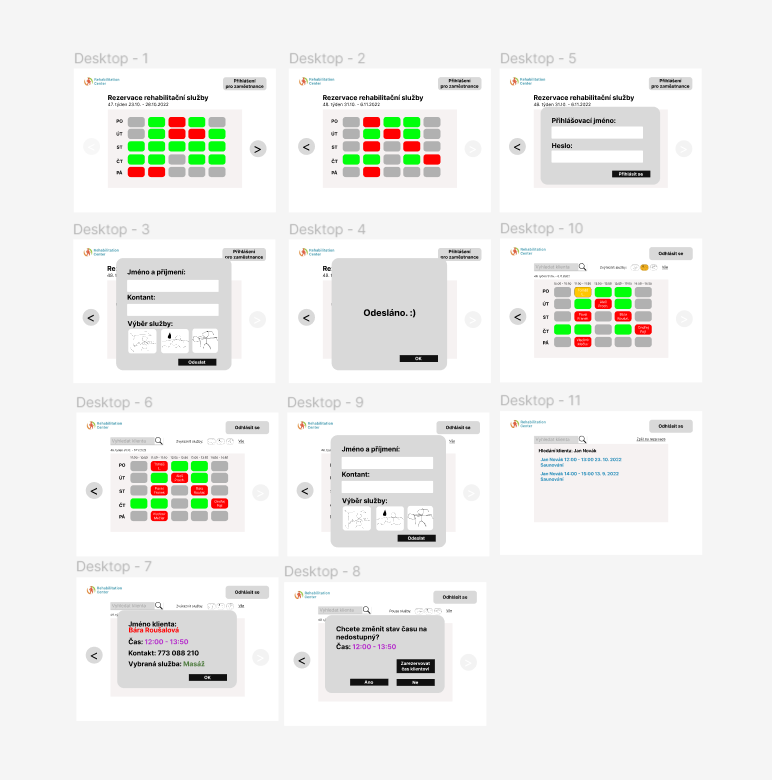
\includegraphics[width = \textwidth]{doc/latex/fig/vit/3.png}
    \caption{Obrázek vytvořeného návrhu rezervačního systému pro Wellness centrum}
    \label{fig:Vit_k2}
\end{figure}

\newpage
\subsubsection*{Testování makety}
Maketa byla aktivně testována na třech uživatelích.\\
Starší uživatel měl problémy se správným pochopení tlačítek, které obsahují text a jeho práce byla pomalejší. Mladší uživatelé zvládli všechny úkoly udělat rychle a snadno se v rezervačním systému orientovali, ač tam byly úplně poprvé. Mladší uživatelé se neptali vůbec. Starší uživatel se často ujišťoval, zda provádí akci správně. Testování makety naštěstí proběhlo úspěšně. 


\newpage

